\section{Interactions issues in Virtual Reality}
\label{theory:interaction-issues}
%**[INTRO IN PROGRESS]**
Virtual Reality brings a new medium with new possibilities, but is not without drawbacks. There are limitations that has to be taken into account when working within the bounds of the medium. The purpose of this section is to highlight the pain-points when designing for VR in order to achieve a better user experience.

\subsection{Generality issues}
%**[INTRO MISSING]**
The selection and design of an interaction for an application is hard to apply to a specific problem or context. From their extensive research about 3D interfaces,Bowman et al. \cite{interactions:Bowman2006} summarize four ways that the majority of interaction techniques exhibit generality:
\begin{enumerate}
  \item Application- and domain-generality: The technique was not designed with any particular application or application domain in mind, but rather was designed to work with any application.
  \item Task-generality: The technique was designed to work in any task situation, rather than being designed to target a specific type of task. For example, the design of a pointing technique (like a ray-cast, see Section \ref{theory:toolsandtech:raycast}) does not take into account the size of the objects to be selected and becomes very difficult to use with very small objects \cite{interaction:Poupyrev1997}.
  \item Device-generality: The technique was designed without consideration for the particular input and display devices that would be used with the technique. Often techniques are implemented and evaluated using particular devices, but the characteristics of those devices are not considered as part of the design process. For example, the HOMER technique\cite{interactions:Bowman1997} is assumed to work with any six DOF input device and any display device, but all of the evaluations of this technique have used a wand-like input device and a head-mounted display (HMD).
  \item User-generality: The technique was not designed with any particular group of users or user characteristics in mind, but rather was designed to work for a "typical" user.
\end{enumerate}

\subsection{Occlusion problem}
\label{theory:interactionissues:occlusion}
A problem with interactions in VR, that has a very small significance on screen-based UI, is occlusion since the user interacts and moves in a VE with 3D objects, the possiblity of objects blocking each other\cite{interactions:cutting1997eye}. To solve this the user can move around in the virtual space and try to find an angle that occludes the object, or use a selection tool (see Section \ref{theory:toolsandtech}) that can be bent around the first object or pass through it. Mossel offers in her study a different solution, where the user can "slice the environment and hide it in order to get access to the desired object\cite{interactions:Mossel2016}.
This method were preferable from the standard method which is to move and find a better angle.
\subsection{Human body limitations}
\label{theory:interactionissues:bodylimits}
One of the main differences with interacting in a virtual environment compared to a screen interface is the importance of the entire human body (not just hands), which brings both opputinities and limitations. This section will shine a light on some major limitations that are important to keep in mind when working with VR interfaces and interactions.
\subsubsection{Fatigue}
Fatigue is one of the biggest problems with VR \cite{limitations:burdea2003virtual}. (Add more content about fatigue)
Selection techniques are more severe on arm and wrist strain/pain while navigation can induce simulation sickness.(expand)
\subsubsection{Reach}
Physical reach is also a big problem when interacting in a virtual environment. It limits the interactionspace to the length of the user's body (most often arms) if the interaction technique is direct manipulation (see Section \ref{theory:toolsandtech:raycast}).
\subsubsection{Field of view}
When working with interfaces on a screen, the designer and the system knows what is visible to the user at any point in time. When diving into VR however, it works the other way around. The user has full control of what is visible at any time, which has to be acounted for. The origin of this the same that we experience everyday in our daily lives, we have information all around us but our vision is restricted to our field of view. The field of view of the user (in VR and the real world, just by moving their eyes) is about 94 degrees in a cone shape (circular vision). Past 77 degrees is considered peripheral vision and is not focusable without turning. The user can rotate their head 30 degrees without any constraint, and max out at 55 degrees. Looking up is 20 degrees as comfortable and 60 as max. Looking down is comfortable to about 12 degrees with a max of 40 degrees. (figure \ref{fig:theory:issues:zones:verti}. By combining all of this we get three directional zones for content (figure \ref{fig:theory:issues:zones}), as explained by Alger in his study about UX for VR \cite{UX:Alger2015}:
\begin{itemize}
  \item \textbf{Main Content zone: 0 - 77\degree} This is the field of view for the user without strain. Usually where the primary UI goes (figure \ref{fig:theory:issues:zones:hori}.a).
  \item \textbf{Peripheral zone 77\degree - 102\degree} The user have to physically strain and turn their head to see this zone. It does still prove suitable for UI of less regulary use (figure \ref{fig:theory:issues:zones:hori}.b).
  \item \textbf{Curiosity zone 102\degree - 158\degree} This zone is only visible when the user rotates their body (figure \ref{fig:theory:issues:zones:hori}.c).
\end{itemize}
There are also 3 depth zones, which represents how the object is percieved. Those are:
\begin{itemize}
\item \textbf{No content zone}: 0 - 50 cm. Alger explains that this is because objects that appear closer than that will cause the user's eyes to cross (figure \ref{fig:theory:issues:zones:hori}.d).
\item \textbf{Primary depth perception zone}: 50cm - 20m. Within these distances the user can perceive objects with depth.
\item \textbf{Beyond the horizon}: 20m - MAX. Objects at this distance loses their depth perspective.
\end{itemize}
By combining three zones that represents where different kinds of content should appear,  Comfort-perifial-curiosity zones can be visualized as well. \cite{UX:Alger2015}

%% BELT UI MAIN UI

\begin{figure}
  \begin{subfigure}{.5\textwidth}
  \centering
  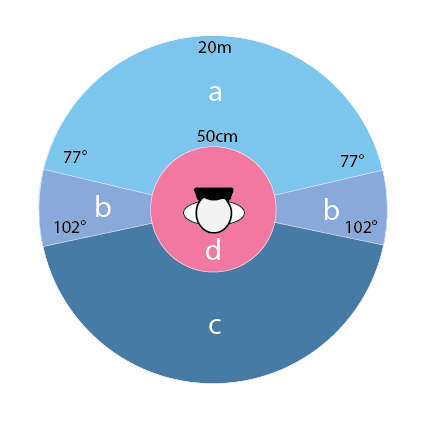
\includegraphics[width=.9\linewidth]{Ergonomic_positions-01.png}
\caption{Horizontal zones used as a guideline when placing content}
\label{fig:theory:issues:zones:hori}
  \end{subfigure}%
  \begin{subfigure}{.5\textwidth}
    \centering
    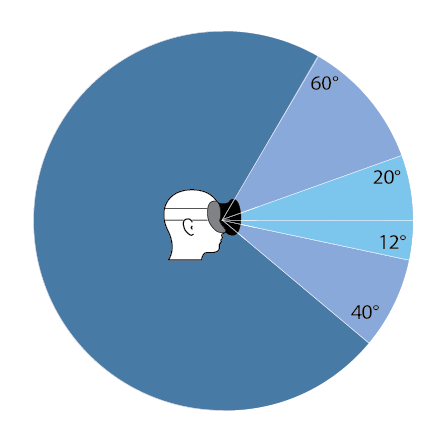
\includegraphics[width=.9\linewidth]{Ergonomic_positions-02.png}
    \caption{Vertical zones that explains human vision restrictions}
    \label{fig:theory:issues:zones:verti}
\end{subfigure}
\caption{Content zones based on research from Alger\cite{UX:Alger2015}}
\label{fig:theory:issues:zones}
\end{figure}



\subsection{Physical Space}
The journey to a virtual environment using a portable headset does not include a vast infinite empty physical space to move around in. This causes problems when users are imerged as they cannot see the physical objects in the real world which can cause and have caused injuries\cite{VR_injuries:2_allen_2017,VR_injuries:steamed}. Some features to the high-end segment to prevent this issue include a visible barrier to inform the user of where to move around freely. This is however something that has to be manually setup before use.\cite{VR_injuries:6_machkovech_2017}
